\chapter{Deep Network}

In recent years, deep learning has succeeded with many applications in different fields. In which, the neural network is the most popular method in deep learning to solve the problem of the high dimensions dataset. This chapter focuses on the discussion about the deep network and its parameters. Firstly, we overview the neural network, its basic components. Secondly, we focus on the main method to update the parameters of neural networks. Thirdly, we mention the objects of this method, dataset. In this part, we will describe the necessary to enlarge the data for the neural network. At the end of this chapter, we present the algorithms that are hired to optimize the learning process.

\section{Deep learning}
Deep learning is known as a part of machine learning. It includes the methods based on learning data representation by allowing the computation on the models that are composed of multiple layers. Each layer extracts the presentation of the input data from the previous layer and computes a new presentation as the input for the next layer. In the hierachy of a deep learning model, the higher layers of representation enlarge aspects of the input that is important for discrimination and suppress irrelevant variations. Each level of representations is corresponding to the different level of abstraction. Deep learning methods work on a large dataset using the backpropagation algorithm to improve the result after each step. The methods of deep learning have effectively improved the results in classification problems \cite{}, object recognition \cite{}, speech recognition \cite{} and other domains \cite{}. 

In deep learning, using neural networks is known as the most popular method. This is a computing-system based on a collection of connected units, called \textit{neurons}. Each neuron has an \textit{activation function} which decides the action that it will be applied to the input (i.e. transfer, drop, \ldots). Each connection (called \textit{synapse}) between the neurons can transmit the signal from a neuron to another neuron. The receiving neuron processes the signal that it received, then it sends the resulting signal to another neuron connected to it. Each connection between neurons is partnered with a weight which manage the important of the input values: It used to increase or decrease the strength of signal that it sends to next units. In practice, the value of weights are initialized randomly. Normally, neurons are organized in layers with different kinds of transformation inside. The signal is travelled multiple times from the first layer to the last layer. The neurons are grouped into three different types of layers: \textbf{input layer, hidden layers and output layer}. The input layer receives input data and then passes the input data to the first hidden layer. The hidden layers make the mathematical computations on their inputs. The last hidden layer gives the output as the input of the output layer. The ``Deep" in Deep learning refers to having more than one hidden layer. The output layer returns the output data of the input.

 

\section{Neural network}
\subsection{Neural}
The basic components of the brain is a neuron. For the ordinary man, we have billion neurons in the human nervous system, and they are connected by the billion of synapses. Each neuron receives input signals from its dendrites and procedures output signals along its axon. At each neuron, the input signals are received, analysed and then given a decision. Fig. \ref{fignneuron} shows the model of a neuron: the left side presents the connections of a biological neuron in human brain, the right side describes the mathematical model at the neuron.

\begin{figure}[h]
	\centering
	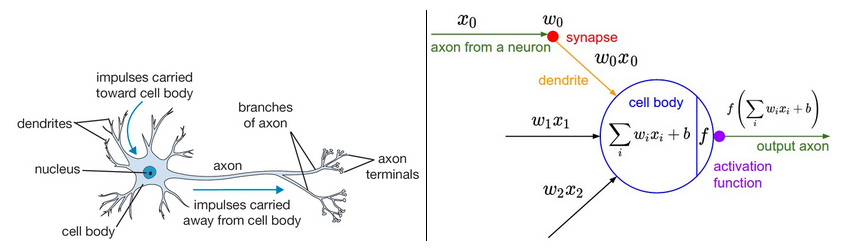
\includegraphics[scale=0.5]{images/neurons.png}
	\caption{A drawing of a biological neuron and its mathematical model}
	\label{fignneuron}
\end{figure}

In the computational model of a neuron, the signals travel along the axons interact multiplicatively with the dendrites of the other neuron based on the synaptic strength at the synapse. The synaptic strength are learnable and control the strength at influence or inhibitory of one neuron on another. In basic mode, the input signals are summed and compared with a threshold value (called \textit{firing rate}). If the sum is greater than threshold value, the neuron can ``fire", sending a spike along its axon. It look likes what we have seen in the real world, the human makes a decision when he take into acount all the conditions. The computation at a neural can be considered as following:
\begin{equation}
	Y = \sum(\text{weight } \ast \text{input}) + \text{bias}
\end{equation}

Depending on the values of the parameters, the output of \textbf{$Y$} can be from $-\infty$ to $+\infty$. So, how do we decide what does a neuron should do in a large range? Should it "fire" or not? Therefore, an ``activation function" has been added to check the value of $Y$ and decide what the neural should be ``fire" (called \textit{activated}) or not.

The first thing in usual is using a threshold for activation function. If the value of $Y$ is greater than the threshold value, the neural will be declared as actived; otherwise, it is not activated. This kind of activation is called \textit{Step} function. It seems that Step function is really work when we would like to create a binary classifier. \textit{For example}, we would like to classify the samples of a dataset includes the samples of two classes (i.e. Class 1 and Class 2). Clearly that Step function works well in this case because it just provides a value to precise a sample will belong to ``Class 1" or ``Class 2". But the problem does not stop there, the question is raised as what will happen if we want to classify more than two classes (i.e three or four classes)? Of course, Step function can still be used in this case if we consider an activated class and other classes are non-activated. But it is really hard to train and converge follows this way. It will be better if we have ``non-binary" activation which can provide the activated (or non-activated) probabilty for each class. The first solution is \textbf{Linear} function. This function gives a range of activations. The user can combine the output of some neurons before deciding. So, that is good too.

However, a neural can not stay alone, it need to connect to other neurons until the last one. In fact, the neurons are organized by the layers and they are connected. If each layer is activated by a linear funtion, the final activation function of the last layer is  just a linear function of the input of the first layer. This means the layers that we have tried to create can be replaced by a single layer. Therefore, we have to use some ``non-linear" activation function in the network if we would like to create a neural network with many layers, i.e. sigmoid, tanh or rectified linear Unit (ReLU).

\textbf{Sigmoid} function is one of the most widely used activation function (Eq. \ref{fsigmoid}). Its output is always going to be in range $(0,1)$.  It means this activation can bound the range of the output instead of $(-\infty, +\infty )$ of linear function. Consider on Eq. \ref{fsigmoid}, if $x$ stays in the range around the origin (i.e $[-2,2]$), then the value of activation has a change being considered. It means any small changes in the values of $x$ in this region will make the output to change significatly. Additional, when $x$ is bigger then $\sigma(x) \rightarrow 1$ and otherwise, $\sigma(x) \rightarrow 0$ if x smaller which means Sigmoid function makes clear distinctions on classification.

\begin{equation}
	\sigma(x) = \frac{1}{1+e^{-x}}
	\label{fsigmoid}
\end{equation}

\textbf{Tanh} is also another popular activation function (Eq. \ref{ftanh}). It is known as a scaled of Sigmoid function (two times Sigmoid). The characteristics of Tanh is similar with the Sigmoid function. However, the output of this functions is zero centered. It means the boundary range is changed to $(-1, 1)$. This point mj 

\begin{equation}
	tanh(x) = 2\sigma(2x) - 1 = \frac{2}{1 + e^{-2x}} - 1
	\label{ftanh}
\end{equation}

\textbf{Rectified Linear Unit (ReLU)} function (Eq. \ref{frelu}) is another activation function which has become in the last of few years. The activation is threshold at zero. At first look this function likes the linear function but in fact they are different because ReLU outputs zero across half its domain. This makes the derivatives through a ReLU remain large and consitent whenever the unit is active. Comparing with Sigmoid or Tanh functions, ReLU was found to greatly accelerate the update parameters of the networks. Addition, ReLU can be easily implemented by threshoding at zero.

\begin{equation}
	f(x) = max(0,x)
	\label{frelu}
\end{equation}

Besides, we have also some generalizations of ReLU such as \textbf{Leaky ReLU} (Eq. \ref{fleakyrelu}), \textbf{PReLU} (Eq. \ref{fPrelu}). They are also more broadly applicable.

\begin{equation}
	f(x) = max(0.01x, x)
	\label{fleakyrelu}
\end{equation}

\begin{equation}
	f(\alpha,x) = max(\alpha x, x)
	\label{fPrelu}
\end{equation}

Actually, we have many kinds of activation functions along with the mentioned functions above. Choosing an activation function for a neuron is depending on the objective of the user when they designed the network. For example, a sigmoid function works well for a classifier because approximating a classifier function as combinations of sigmoid is easier than ReLU for example.

\subsection{Neural network}

\begin{figure}[h]
	\centering
	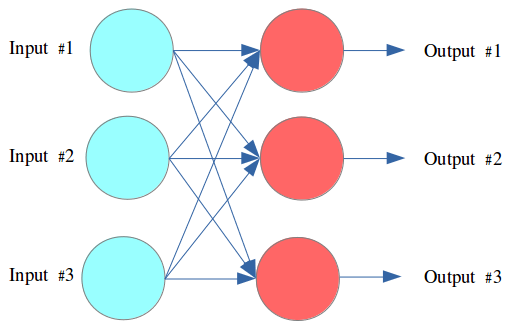
\includegraphics[scale=0.5]{images/neural_net}
	\caption{A model of neural networks}
	\label{fignnnetworks}
\end{figure}

Fig. \ref{fignnnetworks} shows architecture of a simple neural network. The leftmost layer in this network is called the \textit{input layer}, the rightmost layer is called the \textit{output layer}. The neurons within the input layer are called input neurons, the neurons from output layer are called output neurons. When design the network, the input and the output are often straightforward. It means that the neural networks is designed where the output form one layer is used as the input to the next layer, there are no loops in the network, it always feed forward, never feed back (called feedforward networks).

So, the neural network includes many layers are designed as an directred acyclic graph from the intput to the output layer. The output of previous layer is used as the input of the next layer. At each layer excepts the output layer, the output is indicated by a activation function (i.e sigmoid, tanh,...). The size of a neural network can be to compute as the number of neurons, or the number of parameters.

\subsection{Deep network}

A deep neural network is a neural network with multiple layers between the input and the output layers. These layers are called hidden layers. Each layer tries to find the correct mathematical operator to turn its input into the next layer. The deep neural network forwards the data from the input layer to the output layer without looping back: The network creates the connections of neurons and assigns the ``weight" for each connection. At each layer, the weights and its input are multiplied and return an output to transfer to the next layer. Further, an algorithm is used to adjust the weights so that make certain parameters more influential until it receives the correct mathematical manipulation on all dataset. Fig. \ref{figndeepnetworks} presents a deep neural network with multiple hidden layers between the input and the output.

\begin{figure}[h]
	\centering
	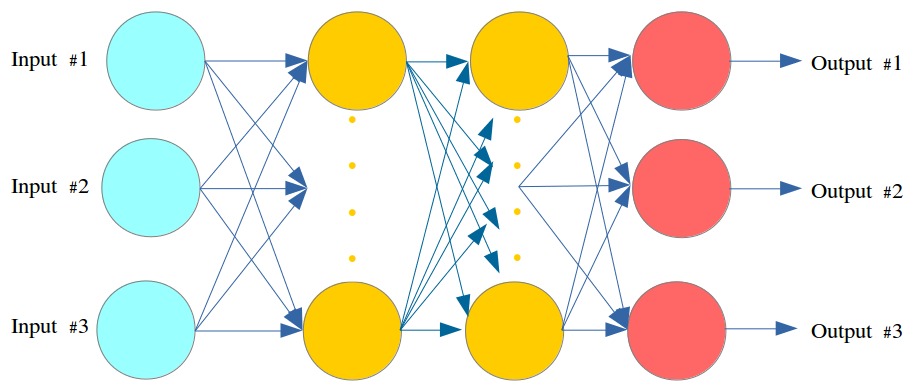
\includegraphics[scale=0.5]{images/deep_neural_network}
	\caption{A deep neural network with multiple hidden layers}
	\label{figndeepnetworks}
\end{figure}

As other machine learning model, designing a deep neural network to solve a problem must be specified an optimization procedure, a cost function and a model family. In deep learning, the gradient-based learning is widely applied because it focus on the difference between the linear models and neural networks. In linear models, the solvers used to train the linear models with global convergence guarantees; instead of, neural network uses gradient-based optimization to drive the cost function to a lowest value after each iteration (because neural network is usually trained by using iterative). Along with gradient-based optimization, a cost fucntion and the represetation of the output of model must be chosen.

A cost function of a neural network is used to compute the difference between the real data and the model's outputs. It is usually updated by each iteration of training process (or validation process). In most of case, we use the cross-entropy between the training data an the model's predictions as the cost function. It means that we define a distribution $p(y | x; \theta)$ and we simply use the priciple of maximum likelihood. But sometimes, we mergely predict some statistic of $y$ conditioned on $x$. The total cost functions of a neural network often combines a primary cost function with a regularization term to make the learning algorithm intend to reduce its generation error.

In our mind, we think that we can separate the choice of the cost function and the output units but in fact, they are related together. For example, if we want to use cross-entropy as the cost function, we need to choose the way to represent the output so that the computing is easy and cheapest. Depending on the solved problem, the output units are chosen to fit with it. For example, we can use the Sigmoid function for a binary classification problem; the Linear function for a transformation with no nonlinearity; the Softmax function for a classifier over \textit{n} different classes.
\section{Back propagation}
A feedforward neural network accepts an input \textbf{$x$} as the initial information, then it was propagated up to the hidden units at each layer and finally procedure an output \textbf{$\hat{y}$}. This is called \textit{forward propagation}. During training, forward propagation can continue until the cost is stable. The \textit{back propagation} algorithm receives the information from the cost (lost function) then flows backward through the network to compute the gradient. This process is repreatedly to discover the gradient for updateing the weights in an attempt to minimize the loss function.

The back-propagation in the form of an algorithm is written as followed:
\begin{enumerate}
	\item \textbf{Input} $x$, \textbf{network} with $L$ layers. Set the corresponding activation $a^1$ for the input layer
	\item \textbf{Feedforward}: For each layer $l = 2, 3, \ldots, L $ compute $z^l = w^la^{l-1} + b^l$ and activation $a^l = \sigma(z^l)$
	\item Compute the error vector: $\delta^L = \nabla_{a}C \odot \sigma'(z^L)$
	\item \textbf{Back-propagation the error}: For each layer $l = L-1, L-2,\ldots, 2$ compute $\delta' = ((w^{l+1})^T \delta^{l+1}) \odot \sigma'(z^l)$
	\item \textbf{Ouput}: the gradient of the cost function given by $\frac{\partial C}{\partial w^l_{jk}} = a^{l-1}_k \delta^l_j$ and $\frac{\delta C}{\delta b^l_j} = \delta^l_j$
\end{enumerate}


The term back-propagation refers only to the method for computing the gradient through recursive application of \textbf{chain rule}. For an arbitrary function $f$, the gradient can be computed from its set of variables whose derivative are desired and set of inputs. It means the process at each function can do independent. In the next, we will describe how to compute the gradient of a function $f(x)$ by using Chain Rule of Calculus which is used to compute the derivaives of functions formed by composing other functions whose derivatives are known.
Let consider a simple multiplication function: $f(x,y) = xy$. The partial derivative of this function as followed:
\begin{equation}
	f(x,y) = xy \rightarrow \frac{\partial f}{\partial x} = y \text{ and } \frac{\partial f}{\partial y} = x
\end{equation}

The objective of derivative is indicating the rate of change of the function with respect to the variable surrounding a small region near a particular point. For example, if $x = 4, y = -3 \rightarrow f(x,y) = -12$, then the derivatives on $x, y$ are:
\begin{equation}
	\frac{\partial f}{\partial x} = -3 \text{ and } \frac{\partial f}{\partial y} = 4
\end{equation}
It means that if we increase the values of $x$, the value of function $f$ will be decreased. Otherwise, if we increase the value of $y$, the ouput of function $f$ is also increased.
For an addition function, the derivatives are:
\begin{equation}
	f(x,y) = x + y \rightarrow \frac{\partial f}{\partial x} = 1 \text{ and } \frac{\partial f}{\partial y} = 1
\end{equation}
And for a MAX operation, the gradient is $1$ on the larger input and $0$ on other inputs:
\begin{equation}
	f(x,y) = max(x,y) \rightarrow \frac{\partial f}{\partial x} = 1 (x \geq y) \text{ and } \frac{\partial f}{\partial y} = 0 (y \geq x)
\end{equation}

Consider example in Fig. \ref{figbackex1}, it presents the function $f(x,y,z) = (x + y)z$. Let see how to apply the derivative to compute the backward pass.

\begin{figure}[h]
	\centering
	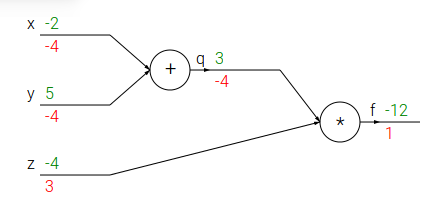
\includegraphics[scale=0.6]{images/back_ex}
	\caption{The computation graph of function $f$}
	\label{figbackex1}
\end{figure}
The \textit{green} values are the input to compute the forward pass. It is very easy to obtain the result: $f(x,y,z) = (x +y)z = (-2 + 5)(-4) = -12$. In the backward pass, the values are computed by applying derivative: At multiply gate, we can easy to compute the gradient of add gate and input $z$ are $-4$ and $3$, respectively. At the add gate, it takes the gradient and multiples it to all of the local gradient for its input. So, the gradient on both $x$ and $y$ are $1 \ast -4 = -4$. Clearly that if we increase the value of $x$ and $y$, the value of add gate will be decreased and it will turn the ouput of multiply gate increase. So, back-propagation can see as gates communicating to each other to make a change on their outputs (decrease or increase) and to make the final value higher.

\section{Data augmentation}

The main problem of machine learning is to make an algorithm that not only perform on the training data but also on new inputs. Many plans have been used in machine learning to reduce the test error but not expense the training cost (re-trainning). A solution is given that the algorithm should be trained on a large dataset where it can covers all the issues of the attented problem.

More of the same, a deep neural network will be better if is is trained with more data. But in practice, we do not always have a large data instead the amount of data is very limitted. A solution for this problem is to create the fake data and add it to the dataset. However, for different tasks, we may be need to apply the different augmentation methods. \textit{For example,} in classification problem, a classifier needs to take a pair of input $x$ and summary it with a single category $y$. This means that the task of a classifier is to be invariant when the input transforms. So, we can generate new $(x,y)$ pairs just by transforming the $x$ inputs in the training set. But this approach is not reality applicable with a \textit{density estimation} task.

Data augmentation has been a particularly effective technique for object recognition problem \cite{}, speech recognition \cite{}. With the operations like translating the images a few pixels some directions, it can often generate the new images. Even the other operations like rotating or scaling the images have also proven effective.

Noise injection can also be as another form of data augmentation \cite{}. For many classification and regression tasks \cite{}, they have proven that the neural network can be improved the robustness when we train them with random noise applied to their input. They are also inserted into the hidden units which can see as an augmentation at multiple levels of consideration. \cite{} shown that this approach can be highly effective provided that the magnitude of the noise is carefully tuned.

Data augmentation is considered as a part of machine learning algorithms. Usually, operations are generally applicable while other operations are specific to one application domain. So, choosing augmentation methods should be thoroughly examined before applying.

\section{Optimization problem}
The optimization for neural networks is a active area, it involves to deep learning in many contexts and one of all is finding the parameters of a neural network that significantly reduce the cost function and improve the accuracy of the algorithm. In the previous section, we have seen how to compute the gradient with back-propagation. They are used to perform the parameters of the network to reduce the cost of the model. There are several appoaches for performing the update. In this section, we present some established and common techniques which have used to optimize the neural networks.

In previous section, we have tried to calculate the gradient of the loss function. Based on that we can compute the best direction along which we should change our weights to guarante the direction of the stepest descent. This process will be repeated to evaluate the gradients and to perform the parameters updating. This procedure is called \textit{Gradient Descent}. The simplest form of this procedure is to change the parameters along the negative direction. Assuming a vector of parameters \textbf{$x$} and the gradient \textbf{$dx$}, the update has the form: 
\begin{equation}
	x = x - learning\_rate \ast dx \text{ (\textbf{learning\_rate} is a fixed constant)}
\end{equation}
A neural network can be trained on a dataset of hundreds of millions of examples. It seems that wasteful to compute the full loss of the network to perform a parameter. So, we can just apply the Gradient descent over \textbf{batches} of training data to achieve the faster convergence. This process is called \textbf{Stochastic Gradient Descent (SGD)}. Using SGD to update training of a minibatch of \textit{m} examples can be described in  Algorithm \ref{sgdalgorithm}.
\begin{algorithm}
	\caption{SGD update at training iteration $k$}
	\label{sgdalgorithm}
	\begin{algorithmic}
		\REQUIRE Learning rate $\epsilon$
		\REQUIRE Initial parameter $\theta$
		\WHILE{stopping criterion not meet}
			\STATE Sample a minibatch of $m$ example from training set $\{ x^1,x^2,\ldots, x^m \}$ with corresponding targets $y^{(i)}$
			\STATE Compute gradient estimate: $\hat{g} \leftarrow + \frac{1}{m} \nabla_\theta \sum_i L(f(x^i;\theta), y^i) $
			\STATE Apply update $\theta \leftarrow \theta - \epsilon \hat{g}$
		\ENDWHILE
	\end{algorithmic}
\end{algorithm}

In SGD algorithm, the learning rate is an important parameter. In previous, the learning rate is fixed as a constant but in practice, it is necessary to decrease the learning rate over time. Denote the learning rate at iteration $k$ as $\epsilon_k$. It is common to decay the learning rate linearly until iteration $\tau$:
\begin{equation}
	\epsilon_k = (1 - \alpha) \epsilon_0 + \alpha \epsilon_\tau
\end{equation}
Where $\alpha = \frac{k}{\tau}$ and after iteration $\tau$, it is common to leave $\epsilon$ constant. Usually, the learning rate is chosen by trial and error. When using the linear schedule, the parameters to choose are $\epsilon_0$, $\epsilon_\tau$, and $\tau$: $\tau$ parameter prefers to the number of iteration after that the learning rate will be decreased, $\epsilon_\tau$ indicates the dropping of the learning rate, the last problem is how to choose the value for initial learning rate $\epsilon_0$. If the learning is too large, the cost function often increases significantly. Otherwise, if the learning rate is too low, the learning process will be slow and learning may become stuck with a high-cost value. Experience indicates that the learning rate in the first $100$ iterations should be higher than the next iterations. Therefore, setting up the first learning rate along with a decreasing schedule should be considered together to obtain the best result.

Besides SGD, the method of momentum \cite{} is designed to accelerate learning. It accumulates an exponentially decaying moving average of past gradients and continues to move in their direction. Acording that, a variable role of velocity $\upsilon$ is introduced, it presents the direction and speed that the parameters move through the parameter space. The velocity is set to an exponentially decaying average of the negative gradient. The SGD algorithm with momentum is describe in Algorithm \ref{sgdm_algorithm}.

\begin{algorithm}
	\caption{SGD with momentum}
	\label{sgdm_algorithm}
	\begin{algorithmic}
		\REQUIRE Learning rate $\epsilon$, momentum parameter $\alpha$
		\REQUIRE Initial parameter $\theta$, initial velocity $\upsilon$
		\WHILE{stopping criterion not meet}
			\STATE Sample a minibatch of $m$ example from training set $\{ x^1,x^2,\ldots, x^m \}$ with corresponding targets $y^{(i)}$
			\STATE Compute gradient estimate: $\hat{g} \leftarrow + \frac{1}{m} \nabla_\theta \sum_i L(f(x^i;\theta), y^i) $
			\STATE Compute velocity update: $\upsilon \leftarrow \alpha \upsilon - \epsilon \hat{g} $
			\STATE Apply update $\theta \leftarrow \theta + \upsilon$
		\ENDWHILE
	\end{algorithmic}
\end{algorithm}

\textbf{Nesterov Momentum} is another version of the momentum on SGD. The difference between Nesterov momentum and standard momentum is where the gradient is evaluated after applying the current velocity. It looks like we add a correlation factor to the standard momentum. The complete Nesterov momentum is presented in Algorithm \ref{sgdNm_algorithm}.

\begin{algorithm}
	\caption{SGD with momentum}
	\label{sgdNm_algorithm}
	\begin{algorithmic}
		\REQUIRE Learning rate $\epsilon$, momentum parameter $\alpha$
		\REQUIRE Initial parameter $\theta$, initial velocity $\upsilon$
		\WHILE{stopping criterion not meet}
			\STATE Sample a minibatch of $m$ example from training set $\{ x^1,x^2,\ldots, x^m \}$ with corresponding targets $y^{(i)}$
			\STATE Apply interim update: $\tilde{\theta} \leftarrow \theta + \alpha \upsilon$
			\STATE Compute gradient: $\hat{g} \leftarrow + \frac{1}{m} \nabla_{\tilde{\theta}} \sum_i L(f(x^i;\tilde{\theta}), y^i) $
			\STATE Compute velocity update: $\upsilon \leftarrow \alpha \upsilon - \epsilon \hat{g} $
			\STATE Apply update $\theta \leftarrow \theta + \upsilon$
		\ENDWHILE
	\end{algorithmic}
\end{algorithm}

The momentum algorithm can accelerate learning and mitigate the issues of the network, but it is expensive of including other hyperparameters. In which, the learning rate is one of the hyperparameters that is the most difficult to set because it has a significant impact on model performance. Tuning the learning rate for each trial is a very expensive process, so adjusting and adapting the learning rate throughout the training phase can be suitable to impale the cost because it is often highly sensitive to the directions in the parameter space. In this part, we highlight some common adaptive methods on learning rate.

\textbf{Delta-bar-delta} algorithm \cite{} is the first approach to adaptive local learning rates for model parameters during training. The algorithm describes that we should increase the learning rate when the partial derivative of the loss with respect the parameters remains the same sign and otherwise, if the partial derivative of the loss with respect the parameters change sign, then the learning rate should decrease. 

\textbf{AdaGrad} algorithm (Algorithm \ref{AdaGrad_algorithm}) adapts the learning rates by scaling them inversely proportional to the square root of the sum of all of their historical squared values. The parameters with the largest parital derivative of the loss have a correspondingly rapid decrease in their learning rate, while parameters with small partial derivatives have a relatively small decrease in their learning rate.

\begin{algorithm}
	\caption{The AdaGrad algorithm}
	\label{AdaGrad_algorithm}
	\begin{algorithmic}
		\REQUIRE Global learning rate $\epsilon$
		\REQUIRE Initial parameter $\theta$
		\REQUIRE Small constant $\delta$ ($i.e. 10^{-7}$)
		\STATE Initialize gradient accumulation variable r = 0
		\WHILE{stopping criterion not meet}
			\STATE Sample a minibatch of $m$ example from training set $\{ x^1,x^2,\ldots, x^m \}$ with corresponding targets $y^{(i)}$
			\STATE Compute gradient: $g \leftarrow + \frac{1}{m} \nabla_{\theta} \sum_i L(f(x^i;\theta), y^i) $
			\STATE Accumulate squared gradient: $r \leftarrow r + g \odot g$
			\STATE Compute update: $\Delta \theta \leftarrow - \frac{\epsilon}{\delta + \sqrt{r}} \odot g$ (Division and square root applied element-wise)
			\STATE Apply update: $\theta \leftarrow \theta + \Delta \theta$
		\ENDWHILE
	\end{algorithmic}
\end{algorithm}

\textbf{RMSProp} algorithm \cite{} (Algorithm \ref{RMSProp_algorithm}) modifies AdaGrad to perform better in non-convex function by chaning the gradient accumulation into an exponentially weighted moving average. 

\begin{algorithm}
	\caption{The RMSProp algorithm}
	\label{RMSProp_algorithm}
	\begin{algorithmic}
		\REQUIRE Global learning rate $\epsilon$, decay rate $\rho$
		\REQUIRE Initial parameter $\theta$
		\REQUIRE Small constant $\delta$ ($i.e. 10^{-6}$)
		\STATE Initialize gradient accumulation variable r = 0
		\WHILE{stopping criterion not meet}
			\STATE Sample a minibatch of $m$ example from training set $\{ x^1,x^2,\ldots, x^m \}$ with corresponding targets $y^{(i)}$
			\STATE Compute gradient: $g \leftarrow + \frac{1}{m} \nabla_{\theta} \sum_i L(f(x^i;\theta), y^i) $
			\STATE Accumulate squared gradient: $r \leftarrow \rho r + (1 - \rho)g \odot g$
			\STATE Compute parameter update: $\Delta \theta \leftarrow - \frac{\epsilon}{\delta + \sqrt{r}} \odot g$ (Division and square root applied element-wise)
			\STATE Apply update: $\theta \leftarrow \theta + \Delta \theta$
		\ENDWHILE
	\end{algorithmic}
\end{algorithm}

\textbf{Adam} algorithm \cite{} (Algorithm \ref{Adam_algorithm}) is another adaptive learning rate optimization. It looks like RMSProp with momentum but in Adam, the momenum is incorporated directly as an estimate of the first order moment of the gradient. Additional, it includes bias corrections to the estimates of both the first-order moments and the second order moments to account for their initialization at the origin.

\begin{algorithm}
	\caption{The Adam algorithm}
	\label{Adam_algorithm}
	\begin{algorithmic}
		\REQUIRE Step size $\epsilon$ (default suggestion $0.001$)
		\REQUIRE Exponential decay rates for moment estimates, $\rho_1, \rho_2$ in $[0, 1)$ (default suggestion $0.9 \text{ and } 0.999$ resprectively)
		\REQUIRE Small constant $\delta$ ($i.e. 10^{-8}$)
		\REQUIRE Initial parameter $\theta$
		\STATE Initialize $1^{st}$ and $2^{nd}$ moment variables $s = 0$, $r = 0$
		\STATE Initialize time step t = 0
		\WHILE{stopping criterion not meet}
			\STATE Sample a minibatch of $m$ example from training set $\{ x^1,x^2,\ldots, x^m \}$ with corresponding targets $y^{(i)}$
			\STATE Compute gradi ent: $g \leftarrow + \frac{1}{m} \nabla_{\theta} \sum_i L(f(x^i;\theta), y^i) $
			\STATE $t \leftarrow t + 1$
			\STATE Update biased first moment estimate: $s \leftarrow \rho_1 s + (1 - \rho_1)g$
			\STATE Update biased second moment estimate: $r \leftarrow \rho_2 r + (1 - \rho_2)g \odot g $
			\STATE Correct bias in first moment: $\hat{s} \leftarrow \frac{s}{1-\rho_1^t}$
			\STATE Correct bias in second moment: $\hat{r} \leftarrow \frac{r}{1 - \rho_2^t}$
			\STATE Compute parameter update: $\Delta \theta \leftarrow - \epsilon \frac{\hat{s}}{\sqrt{\hat{r} + \delta}} \odot g$ (Division and square root applied element-wise)
			\STATE Apply update: $\theta \leftarrow \theta + \Delta \theta$
		\ENDWHILE
	\end{algorithmic}
\end{algorithm}

In this section, we have described a highlight algorithms related to optimize the deep models by adapting the learning rate for each model parameter. The question is what algorithm should we choose? There is currently no consensus on this point. Choosing an algorithm is depending on the user's familiarity with the algorithm. In practice, the most popular algorithms are used include  SGD, SGD with momentum, RMSProp, and Adam.

\section{Conclusion}
In this chapter, we have described the basic components of deep learning by using the neural network. Using any algorithms for deep learning is depending on the users but generally, the problems that we have mentioned are indispensable \textit{i.e.} designing the algorithm, optimization problem. This chapter just provides to us a generally understood about deep learning but it is really important to help us have the first overviews about a method in this field before going to the further. In the next, we will enter into another method on deep learning, Convolutional Neural Network, and then is its application to predicting landmark on the beetle dataset.